
\section{\uppercase{Signal Quantization For Rapid Classification}}
\label{sec:quantization}

%We are interested in minimizing computational expense of classifying mental gestures. This study investigates a signal quantization technique that reduces the size of EEG data for fast classification but retains high accuracy.

\noindent Our objective is to maximize the accuracy of the classifier while minimizing its computational expense. One way to reduce the computational requirements of a classifier is to reduce the size of the feature vectors on which it is trained and tested. We propose a signal quantization method that allows us to directly adjust the size of feature vectors by changing the signal's resolution. This allows us to operationalize a tradeoff between the running time and accuracy of the classifier.

%Generally, we seek to maximize our system's classification accuracy while minimizing its computational expense. One way to reduce the computational requirements of a SVM classifier is to reduce the size of the feature vectors on which it is trained and tested. Our signal quantization method allows us to directly adjust the size of feature vectors by changing the signal's resolution (see 3.1), though lowering the resolution of feature vectors could negatively effect the classifier's performance.

%\subsection{Compressing power spectra in the temporal dimension}

We compress the power spectrum time series in the temporal dimension. Given a sequence of 20 power spectra (from a 10 second trial), with 1024 frequency components per spectrum, we compute a discrete probability density function (pdf) in which each component is the mean of its corresponding frequency components through time. This results in a discrete pdf with 1024 components for each trial.

%First, we compute an average of all the power spectra associated with a recording. We obtain a discrete probability density function (PDF) in which each bin is the mean of its corresponding bins through time. At this stage, we have a discrete PDF of 1024 bins for the entire n second recording. 

\subsection{Logarithmic Binning}

Since EEG activity is associated with frequencies from 1-40Hz, we presume this range contains the majority of relevant signal. However, this frequency range can be polluted with non-neural signals \cite{ball2009signal}, and we do not rule out the possibility that useful signal exists in other frequency ranges as well. Muscular activity, for example, might be correlated with mental gestures in some cases. In order to exploit the entire frequency spectrum while preserving our bias toward known sources of useful signal, we select a logarithmic spacing of the data bins through the pdf. Figure \ref{binnedEEGpowerspec} shows an example of logarithmic binning with 100 bins. It offers a 10x compression ratio while still preserving the structure of the original 1024-point pdf.

We apply the quantization step by performing data binning on the probability density function. Data binning offers a simple way to ``quantize'' the information contained in the full signal. By taking the mean of several adjacent points in the pdf, we are left with a single bin that compresses the information contained in its local area of frequencies. For instance, four contiguous frequencies (1Hz, 1.25Hz, 1.5Hz, 1.75Hz) of the values (4, 4, 5, 5) could be combined into a single bin with the value 4.5. The number of bins can be chosen to provide a desired level of  resolution on the signal.

%Binning a probability density function (PDF) is a simple way to ``quantize'' the information contained in the full signal. By taking the mean of several adjacent points in the PDF, we are left with a single bin that compresses the information contained in its local area of frequencies. For instance, four contiguous frequencies (1, 1.25, 1.5, 1.75) of the values (4,4,5,5) could be combined into a single bin with the value 4.5. 

\begin{figure}[!h]
  \vspace{-0.2cm}
  \centering
  {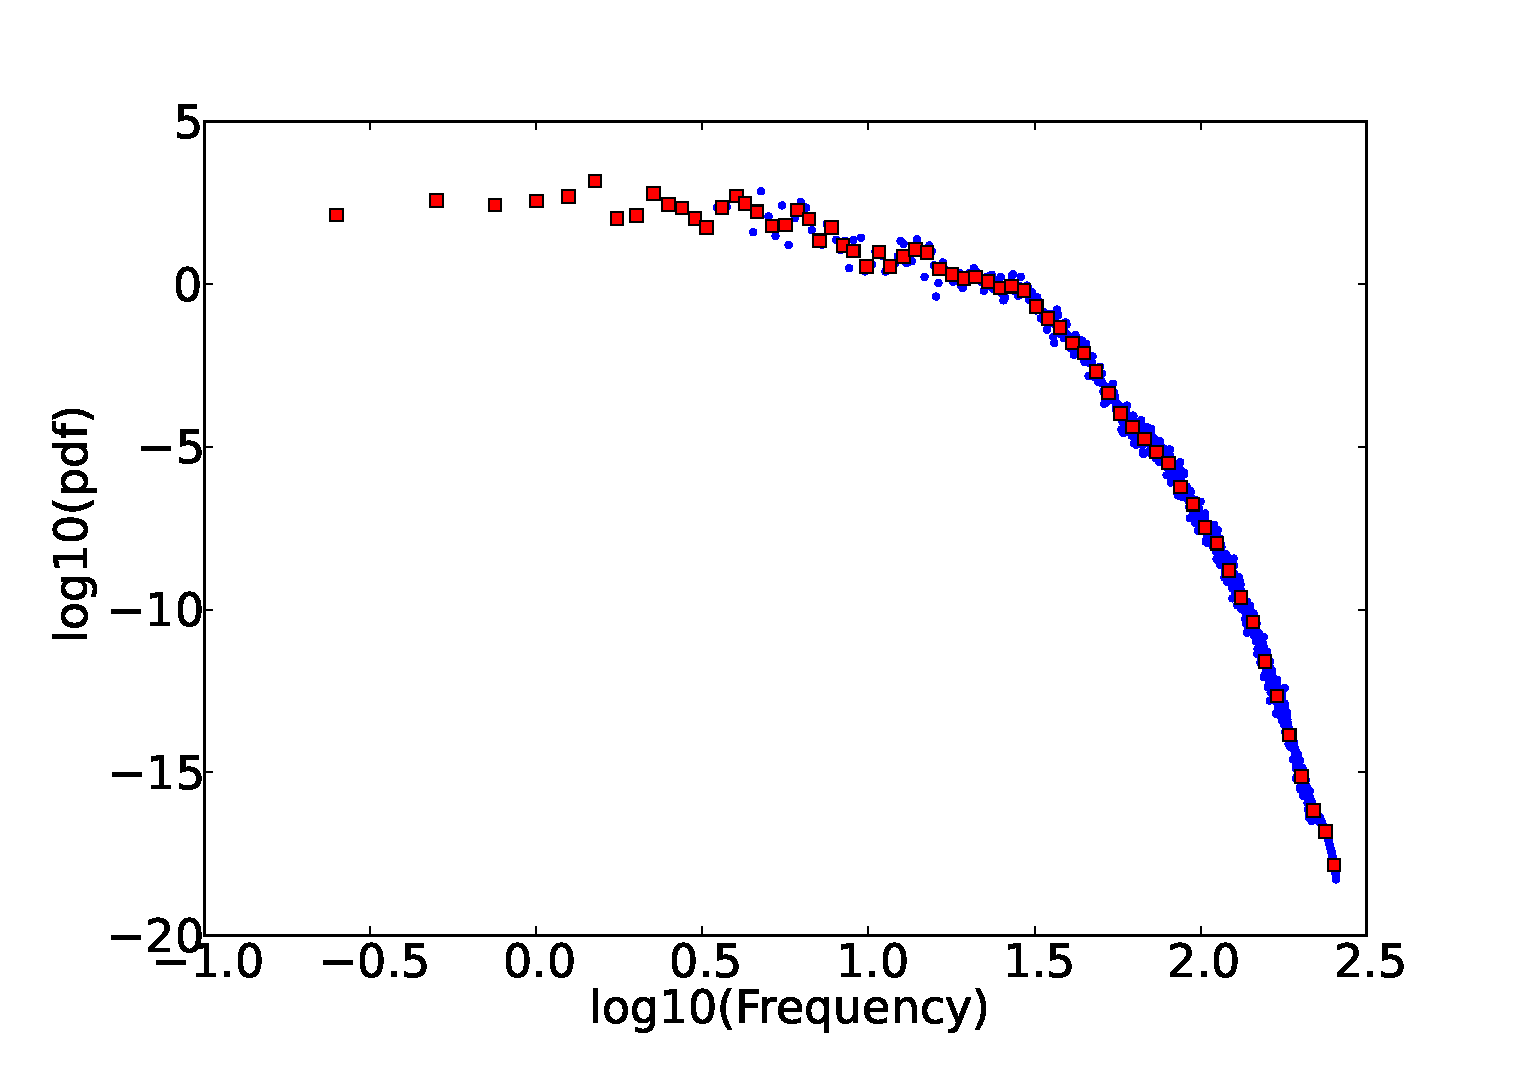
\epsfig{file = Figures/figure1.eps, width = 8cm}}
\caption{In double logarithmic scale, the original 1024 bins (blue dots) of the probability density function (pdf) obtained from averaging the \emph{n} power spectra of one recording, and the resulting ``quantized''  pdf with a resolution of 100 log-bins (red dots). The quantized pdf preserves very well the structure of the original, 1024-point pdf. }
\label{binnedEEGpowerspec}
\vspace{-0.1cm}
\end{figure}

%In summary, we build a probability density function of frequencies captured by the EEG scanning device from all the power spectra in a recording. We then use logarithmically-spaced bins to reduce the original 1024 frequency values to a smaller number of bins (e.g., 100 log-bins in \ref{binnedEEGpowerspec}). This method produces a statistical average of a time series, compressed into a single feature vector that it is easy to use in a classifier.

The output of the logarithmic binning step is a single feature vector, whose size is controlled by the number of bins. This vector can now be used as an input into the classifier.

\subsection{Binary BCI Classifier}

To test the performance of the quantization method, we build a binary BCI using a support vector machine (SVM) classifier, which we train individually on each subject's recordings while varying the bin size. We use LinearSVC \cite{fan_liblinear:_2008}, a wrapper for LibLinear exposed in Python through the scikit-learn library \cite{pedregosa_scikit-learn:_2011}. We chose LinearSVC because BCI classification problems are generally presumed to be linear  \cite{garrett_comparison_2003,lotte_review_2007}, and because LibLinear's underlying C implementation boasts among the fastest train- and test-time performance among state-of-the-art solutions \cite{fan_liblinear:_2008}. We use a hyperparameter of 100, found through a ``grid search'', or an exhaustive search through a randomly-selected sample of our dataset. 
%When training a classifier, the only way to make accurate estimates of the classifier's performance is to test it on data on which the classifier was not trained. A common way to do this is through \textit{cross-validation}, in which we train and test a classifier several times using different subsets of the data for training and testing. 
We use scikit-learn's built-in cross-validation toolkit, which performs seven cross-validation steps using different splits of data in each round.

%\subsection{Creating a binary BCI}

Out of the seven mental gestures in the dataset, we want to identify and select, for each individual subject, the two best gestures for that subject. This will result in a personalized binary (two-class) classifier, where the SVM can discriminate between two mental gestures performed by the subject with the highest classification accuracy. The gesture-pairs may vary from subject to subject. For example, one subject's best-case pair may be \textit{song} and \textit{sport} while another's may be \textit{color} and \textit{finger}.

%A binary BCI allows users to select one of two options. In our system, have a ``vocabulary'' of two mental gestures, and our SVM discriminates which gesture they are performing in a given recording. Thus, for any given user, we are interested in finding two tasks between which our SVM can reliably discriminate. This task-pair differs between subjects: one subject's best-case task-pair may be \textit{song} and \textit{sport} while another's could be \textit{eye} and \textit{finger}. 

% Question: for each task, we have 20 trials of 10 seconds each, so total should be 200 seconds, right??

%In order to simulate a binary BCI with our dataset, we spliced all mental task recordings into $\sfrac{1}{2}$-second chunks, each one representing a single power spectrum reading from our headset. In Section 5, we simulate calibrating the BCI to a taskpair by cross-validating an SVM trained on all taskpair data. In Section 6, we use a more realistic approach in which we train the SVM on the first eighty seconds of data for both tasks, then testing the classifier on the remaining 40 seconds of data.

% {\bf NB:} I believe that the classifier does well because it can efficiently capture the overall level of activity for all log-bins, but also more local deviations. On the figure, we can see some local peaks mostly between $10^1$ and $10^1.5$, but in all other parts of the PDF though in a less visible way. I believe these deviations are quite unique and can make the difference in the classifier. We should indeed check this further if we want to understand to origins of the good results.

% {\bf Side note:} one way to investigate further would be to see indeed to what extent the ``compression", i.e. the small number of log-bins, affects the quality of the classifier. Another quite promising further research direction, would be to determine the minimum number of n power spectra, which should be taken into account to reach a target level of correct classification. This would be useful to determine what should be the most adequate sample size for a certain level of identification. This level might of course vary as a function of subjects and tasks.

%-----------


% \textcolor{red}{\bf [Maybe a schema would be great to help the reader get the point quickly]}
